\chapter{Taylormodelle}

Ein Taylormodell, in \cite{makino2001} eingeführt und in \cite{DBLP:conf/macis/BrausseKM15} erweitert, ist ein Polynom $T = \sum_n c_n \lambda^n$, mit $k$ Variablen. $\lambda_i$ ist ein Fehlersymbol aus $\lambda = (\lambda_1, ... , \lambda_k)$, dem Vektor der Fehlersymbole, wodurch funktionale Abhängigkeiten zwischen Monomen und anderen Taylormodellen hergestellt werden können. Die Koeffizienten des Polynoms sind Intervalle $c_i = [\Tilde{c}_i \pm e_i] \subseteq \mathbb{R}$ mit denen der aktuelle Rechenfehler ('approximation error') abgeschätzt wird. Ist ein Wert genau bekann, also ohne Ungenauigkeit oder Fehler, kann dieser als Punktintervall mit $c_i = [\Tilde{c}_i \pm 0]$ definiert werden, also mit einem Zentrum ohne Radius.


\section{Darstellung}
Ein Taylormodell besteht in der Implementierung aus dem Kernintervall \verb+kernel+, einer Liste von sortierten von Monomen und einer Liste von Supportintervallen, den Intervallen, der Fehlersymbole. Die Liste der Supportintervalle ist für jedes Taylormodell dieselbe.


\section{Spezielle Operationen auf Taylormodellen}
\paragraph{Quadratisches Sweeping}
Um die Länge der Polynome und deren Grad in den Taylormodellen zu kontrollieren können einzelne 
Fehlersymbole in einem Monom durch ihr Intervall ersetzt werden. So erhöht sich zwar die Breite des 
Koeffizienten, allerdings wird auch das Verrechnen mit einem anderen, nun gleichen Monom 
ermöglicht. Dieses \textit{Sweeping} bietet eine natürliche Möglichkeit, den durch die 
Fehlersymbole eingeführten Fehler klein zu halten, indem versucht wird, bei
\textit{quadratischen} Terme nicht ein Fehlersymbol nach dem anderen zu Sweepen, sondern deren 
Quadrate einzusetzen: \par
Gegeben sei ein Monom eines Polynoms $...+ c \cdot \lambda^3 + ...$ mit $\lambda \in [-1.5, 1.5]$. Nun sieht man, dass zwar $\lambda$ sowohl positiv, als auch negativ sein kann, jedoch das Quadrat nicht. Daher kann man statt
\begin{align*}
    & ... + c \cdot \lambda^3 + ... \\
    \rightarrow & ...+ c \cdot [-1.5, 1.5] \cdot \lambda^2  +... \\
    \rightarrow & ...+ c \cdot [-1.5, 1.5] \cdot [-1.5, 1.5] \cdot \lambda +... \\
    \rightarrow & ...+ c \cdot [-2.25, 2.25] \cdot \lambda+... \\
\end{align*}
das Quadrat einsetzen
\begin{align*}
    & ... + c \cdot \lambda^3 + ... \\
    \rightarrow & ...+ c \cdot [0, 2.25] \cdot \lambda +...
\end{align*}
und somit das Wachstum des Rechenfehlers verlangsamen. 
\paragraph{Polishing}
Rechenoperationen auf Intervallen sorgen dafür, dass sich diese Vergrößern. Mit gut gewählten Sweeping-Stategien kann dieser Effekt zwar verlansamt, aber nicht aufgehalten werden. Wie in Kapitel \ref{ch:Evaluierung} zu sehen ist, kann ab einer bestimmten Intervallbreite keine 
Aussage mehr über das Ergebnis getroffen werden. Mit \textit{Polishing} \cite{DBLP:conf/macis/BrausseKM15} kann ein zu großes Intervall eines Koeffizienten in zwei Monome mit jeweils einem Punktintervall und einem neuen Fehlersymbol aufgeteilt werden. Das verlängert zwar das Polynom, verhindert jedoch ein zu großes Wachstum der Intervallbreite. Eine Implementierung in \verb+hotm+ ist  derzeit nicht vorhanden, aber angedacht.


\section{Sweeping-Strategien}
In einer linearen Implementierung der Taylormodelle und deren Polynome, muss Sweeping in jeder Multiplikation geschehen, da sich sonst der Grad des Polynome erhöhte. Folgt man der Idee des \textit{quadratischen Sweepens}, so ergibt sich bei der Multiplikation zweier Polynome und dementsprechend der paarweisen Multiplikation der Monome: 
$$(c_1 \cdot \lambda_i) \cdot (c_2 \cdot \lambda_j) = \begin{cases}

c_1 c_2 s_j \lambda_i & \text{wenn } i \neq j \text{ und } s_i > s_j \\
c_1 c_2 s_i \lambda_j & \text{wenn } i \neq j \text{ und } s_i \leq s_j \\
c_1 c_2 s_i^2 & \text{wenn } i = j
\end{cases} \quad \quad \lambda_i \in s_i, \lambda_j \in s_j $$

Im dritten Fall, also bei $i = j$, wird das Ergebnis der Multiplikation zum Kernintervall addiert. Das Problem bei dieser Herangehensweise ist, dass ein Fehler, der ins Kernintervall gesweept wurde, nicht mehr mit einem Fehlersymbol ($\lambda$) assoziiert werden kann und damit keinerlei Abhängigkeitsinformationen mehr enthält. Zwar tritt dieser Fall nicht so häufig auf, wie die beiden anderen, allerdings bedeutet das auch, dass nicht so häufig quadratisch gesweept wird. Eine nicht-lineare Implementierung erlaubt ein Wachsen der Grade der Polynome und andere Sweeping-Strategien. In \verb+hotm+ geschieht das Sweeping eines Taylormodells \textit{t} per Funktionsaufruf unter Angabe der zu verwendenden Sweeping-Strategie und dem Grad, auf den \textit{t} reduziert werden soll. Wird beispielsweise als Grad \glqq 1\grqq\ mitgegeben, ist die Ausgabe höchstens linear, es werden also keine Monome auf den Grad 0 reduziert. Um ein Taylomodell zu evaluieren und auf ein einziges Intervall zu reduzieren, muss der Zielgrad \glqq 0\grqq\ sein.

\begin{algorithm}
\SetAlgoLined
\label{algo:mult}
\SetKwInOut{Input}{input}
\Input{Taylormodell $t$, Grad $deg$, Strategie $strat$}
$Polynomial\ p \gets [\ ]$\;
\ForEach{$Monomial\ m \in t.polynomial$}{
    $rest \gets degree(m) - deg $\;
    \uIf{$rest < 1$} {
        $p.insert(m)$\;
    } \uElse{
        \ForEach{$ErrorSymbol\ es \in m$}{
            \uIf{rest < threshold}{
                break\;
            }
            Sweep according to Strategy\;
            $rest \gets rest - \text{amount swept}$\;
        }
        $p.insert(m)$\;
    }
    
}


\Return $t$

 \caption{Sweeping eines (nicht-linearen) Taylormodells}
\end{algorithm}

Da sich der Grad eines Polynoms nach dem Grad des größten Monoms richtet, muss jedes Monom auf den Zielgrad reduziert werden. Dafür wird über die Fehlersymbole der einzelnen Monome iteriert und eine der Strategien angewandt:

\paragraph{square\_only}
Das Sweeping wird auf quadratisches Sweeping beschränkt. Für jedes Fehlersymbol mit einem Exponenten $> 1$ wird versucht, einen möglichst großen, geraden Wert von demselben abzuziehen. \\
\textbf{Beispiel sweep\_to(1):}
\begin{align*}
   ...+ c \cdot \lambda_1^2 \lambda_2^5 \lambda_3^1 +... & \quad (\lambda_i \in s_i) \\
    ...+ cs_1^2 \cdot \lambda_2^5 \lambda_3^1 +... & \quad \lambda_1 \text{ wird quadriert und somit quasi weggekürzt} \\
    ...+ cs_1^2s_2^{2^2} \cdot \lambda_2^1 \lambda_3^1 +... & \quad \lambda_2 \text{ kann nur 2-mal quad. gesweept werden}
\end{align*}
Unter Verwendung von \verb+square_only+ ist es möglich, dass das Ergebnis, wie im Beispiel, nicht den angegebenen Zielgrad erreicht. 


\paragraph{square\_first / simple}
Hier wird zunächst \verb+square_only+ auf das Monom angewandt, um danach die restlichen Grade ohne quadratisches Sweeping zu reduzieren. Allerdings hat diese Methode keinerlei Vorteile gegenüber \verb+simple+, da der Effekt des Quadrierens von einem nicht-quadratischen Sweep wieder aufgehoben wird.




% \begin{figure}[ht]
    \centering
    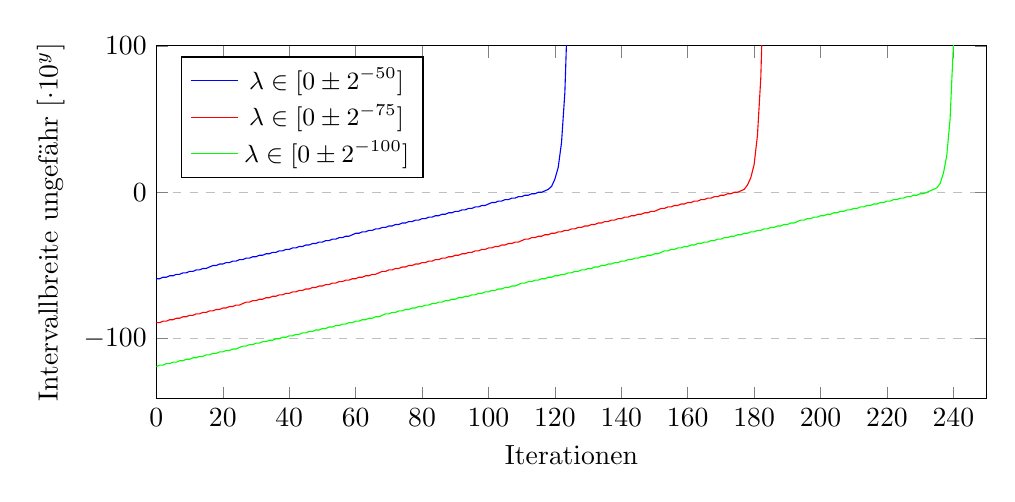
\begin{tikzpicture}
    \begin{axis}[
    width=\textwidth,
    height=0.5\textwidth,
        xlabel={Iterationen},
        ylabel={Intervallbreite ungefähr $[\cdot 10^y ]$},
        legend pos=north west,
        xmin=0,xmax=250,
        ymax=100,
        ymajorgrids=true,
        grid style=dashed,
    ]
    \addplot[
        color=blue,
        ]
        coordinates {
(0,-59) (1,-59) (2,-58) (3,-58) (4,-57) (5,-57) (6,-56) (7,-56) (8,-55) (9,-55) (10,-54) (11,-54) (12,-53) (13,-53) (14,-52) (15,-52) (16,-51) (17,-50) (18,-50) (19,-49) (20,-49) (21,-48) (22,-48) (23,-47) (24,-47) (25,-46) (26,-46) (27,-45) (28,-45) (29,-44) (30,-44) (31,-43) (32,-43) (33,-42) (34,-42) (35,-41) (36,-41) (37,-40) (38,-40) (39,-39) (40,-39) (41,-38) (42,-38) (43,-37) (44,-37) (45,-36) (46,-36) (47,-35) (48,-35) (49,-34) (50,-34) (51,-33) (52,-33) (53,-32) (54,-32) (55,-31) (56,-31) (57,-30) (58,-30) (59,-29) (60,-28) (61,-28) (62,-27) (63,-27) (64,-26) (65,-26) (66,-25) (67,-25) (68,-24) (69,-24) (70,-23) (71,-23) (72,-22) (73,-22) (74,-21) (75,-21) (76,-20) (77,-20) (78,-19) (79,-19) (80,-18) (81,-18) (82,-17) (83,-17) (84,-16) (85,-16) (86,-15) (87,-15) (88,-14) (89,-14) (90,-13) (91,-13) (92,-12) (93,-12) (94,-11) (95,-11) (96,-10) (97,-10) (98,-9) (99,-9) (100,-8) (101,-7) (102,-7) (103,-6) (104,-6) (105,-5) (106,-5) (107,-4) (108,-4) (109,-3) (110,-3) (111,-2) (112,-2) (113,-1) (114,-1) (115,0000) (116,0000) (117,0001) (118,0002) (119,0004) (120,0009) (121,0017) (122,0034) (123,0068) (124,0137) (125,0273) (126,0547) (127,1093) (128,2187) (129,4373) (130,8746)
        };
        \addlegendentry{\small{$\lambda \in [0 \pm 2^{-50}]$}}
        
    \addplot[
        color=red,
        ]
        coordinates {
(0,-89) (1,-89) (2,-88) (3,-88) (4,-87) (5,-87) (6,-86) (7,-86) (8,-85) (9,-85) (10,-84) (11,-84) (12,-83) (13,-83) (14,-82) (15,-82) (16,-81) (17,-81) (18,-80) (19,-80) (20,-79) (21,-79) (22,-78) (23,-78) (24,-77) (25,-77) (26,-76) (27,-75) (28,-75) (29,-74) (30,-74) (31,-73) (32,-73) (33,-72) (34,-72) (35,-71) (36,-71) (37,-70) (38,-70) (39,-69) (40,-69) (41,-68) (42,-68) (43,-67) (44,-67) (45,-66) (46,-66) (47,-65) (48,-65) (49,-64) (50,-64) (51,-63) (52,-63) (53,-62) (54,-62) (55,-61) (56,-61) (57,-60) (58,-60) (59,-59) (60,-59) (61,-58) (62,-58) (63,-57) (64,-57) (65,-56) (66,-56) (67,-55) (68,-54) (69,-54) (70,-53) (71,-53) (72,-52) (73,-52) (74,-51) (75,-51) (76,-50) (77,-50) (78,-49) (79,-49) (80,-48) (81,-48) (82,-47) (83,-47) (84,-46) (85,-46) (86,-45) (87,-45) (88,-44) (89,-44) (90,-43) (91,-43) (92,-42) (93,-42) (94,-41) (95,-41) (96,-40) (97,-40) (98,-39) (99,-39) (100,-38) (101,-38) (102,-37) (103,-37) (104,-36) (105,-36) (106,-35) (107,-35) (108,-34) (109,-34) (110,-33) (111,-32) (112,-32) (113,-31) (114,-31) (115,-30) (116,-30) (117,-29) (118,-29) (119,-28) (120,-28) (121,-27) (122,-27) (123,-26) (124,-26) (125,-25) (126,-25) (127,-24) (128,-24) (129,-23) (130,-23) (131,-22) (132,-22) (133,-21) (134,-21) (135,-20) (136,-20) (137,-19) (138,-19) (139,-18) (140,-18) (141,-17) (142,-17) (143,-16) (144,-16) (145,-15) (146,-15) (147,-14) (148,-14) (149,-13) (150,-13) (151,-12) (152,-11) (153,-11) (154,-10) (155,-10) (156,-9) (157,-9) (158,-8) (159,-8) (160,-7) (161,-7) (162,-6) (163,-6) (164,-5) (165,-5) (166,-4) (167,-4) (168,-3) (169,-3) (170,-2) (171,-2) (172,-1) (173,-1) (174,0000) (175,0000) (176,0001) (177,0002) (178,0005) (179,0010) (180,0019) (181,0039) (182,0078) (183,0156)



        };
        \addlegendentry{\small{$\lambda \in [0 \pm 2^{-75}]$}}
    
        
\addplot[
        color=green,
        ]
        coordinates {
        (0,-119) (1,-118) (2,-118) (3,-117) (4,-117) (5,-116) (6,-116) (7,-115) (8,-115) (9,-114) (10,-114) (11,-113) (12,-113) (13,-112) (14,-112) (15,-111) (16,-111) (17,-110) (18,-110) (19,-109) (20,-109) (21,-108) (22,-108) (23,-107) (24,-107) (25,-106) (26,-105) (27,-105) (28,-104) (29,-104) (30,-103) (31,-103) (32,-102) (33,-102) (34,-101) (35,-101) (36,-100) (37,-100) (38,-99) (39,-99) (40,-98) (41,-98) (42,-97) (43,-97) (44,-96) (45,-96) (46,-95) (47,-95) (48,-94) (49,-94) (50,-93) (51,-93) (52,-92) (53,-92) (54,-91) (55,-91) (56,-90) (57,-90) (58,-89) (59,-89) (60,-88) (61,-88) (62,-87) (63,-87) (64,-86) (65,-86) (66,-85) (67,-85) (68,-84) (69,-83) (70,-83) (71,-82) (72,-82) (73,-81) (74,-81) (75,-80) (76,-80) (77,-79) (78,-79) (79,-78) (80,-78) (81,-77) (82,-77) (83,-76) (84,-76) (85,-75) (86,-75) (87,-74) (88,-74) (89,-73) (90,-73) (91,-72) (92,-72) (93,-71) (94,-71) (95,-70) (96,-70) (97,-69) (98,-69) (99,-68) (100,-68) (101,-67) (102,-67) (103,-66) (104,-66) (105,-65) (106,-65) (107,-64) (108,-64) (109,-63) (110,-62) (111,-62) (112,-61) (113,-61) (114,-60) (115,-60) (116,-59) (117,-59) (118,-58) (119,-58) (120,-57) (121,-57) (122,-56) (123,-56) (124,-55) (125,-55) (126,-54) (127,-54) (128,-53) (129,-53) (130,-52) (131,-52) (132,-51) (133,-51) (134,-50) (135,-50) (136,-49) (137,-49) (138,-48) (139,-48) (140,-47) (141,-47) (142,-46) (143,-46) (144,-45) (145,-45) (146,-44) (147,-44) (148,-43) (149,-43) (150,-42) (151,-42) (152,-41) (153,-40) (154,-40) (155,-39) (156,-39) (157,-38) (158,-38) (159,-37) (160,-37) (161,-36) (162,-36) (163,-35) (164,-35) (165,-34) (166,-34) (167,-33) (168,-33) (169,-32) (170,-32) (171,-31) (172,-31) (173,-30) (174,-30) (175,-29) (176,-29) (177,-28) (178,-28) (179,-27) (180,-27) (181,-26) (182,-26) (183,-25) (184,-25) (185,-24) (186,-24) (187,-23) (188,-23) (189,-22) (190,-22) (191,-21) (192,-21) (193,-20) (194,-19) (195,-19) (196,-18) (197,-18) (198,-17) (199,-17) (200,-16) (201,-16) (202,-15) (203,-15) (204,-14) (205,-14) (206,-13) (207,-13) (208,-12) (209,-12) (210,-11) (211,-11) (212,-10) (213,-10) (214,-9) (215,-9) (216,-8) (217,-8) (218,-7) (219,-7) (220,-6) (221,-6) (222,-5) (223,-5) (224,-4) (225,-4) (226,-3) (227,-3) (228,-2) (229,-2) (230,-1) (231,-1) (232,0000) (233,0001) (234,0002) (235,0003) (236,0006) (237,0013) (238,0025) (239,0050) (240,0101) 


        };
        \addlegendentry{\small{$\lambda \in [0 \pm 2^{-100}]$}}
    
    \end{axis}
    \end{tikzpicture}
    \caption{Größenordnung der Breite des Kernintervalls bei der Berechnung von $x_{250}$ mit Sweeping simple}
    \label{fig:strategy}
\end{figure}

% 
\begin{figure}[ht]
    \centering
    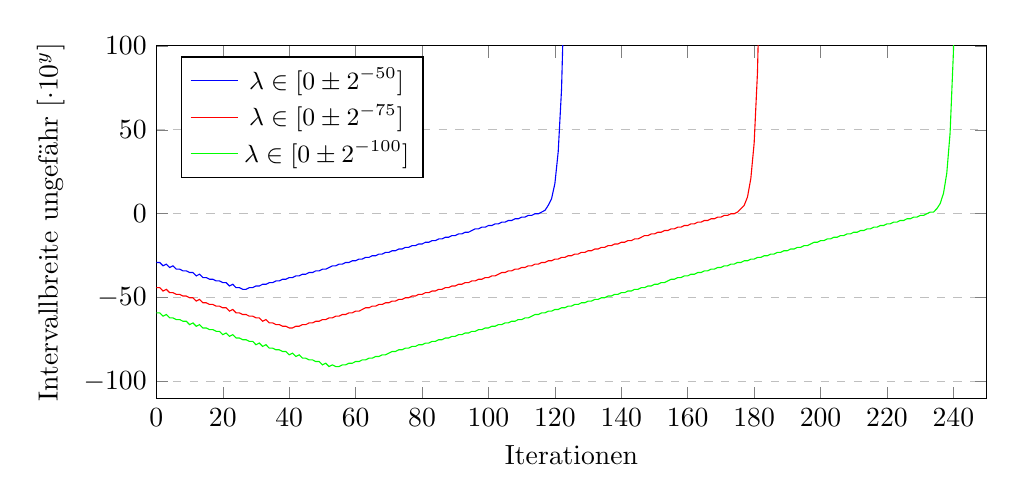
\begin{tikzpicture}
    \begin{axis}[
    width=\textwidth,
    height=0.5\textwidth,
        xlabel={Iterationen},
        ylabel={Intervallbreite ungefähr $[\cdot 10^y ]$},
        legend pos=north west,
        xmin=0,xmax=250,
        ymax=100,
        ymajorgrids=true,
        grid style=dashed,
    ]
    
    \addplot[
        color=blue,
        ]
        coordinates {
 (0,-29) (1,-29) (2,-31) (3,-30) (4,-32) (5,-31) (6,-33) (7,-33) (8,-34) (9,-34) (10,-35) (11,-35) (12,-37) (13,-36) (14,-38) (15,-38) (16,-39) (17,-39) (18,-40) (19,-40) (20,-41) (21,-41) (22,-43) (23,-42) (24,-44) (25,-44) (26,-45) (27,-45) (28,-44) (29,-44) (30,-43) (31,-43) (32,-42) (33,-42) (34,-41) (35,-41) (36,-40) (37,-40) (38,-39) (39,-39) (40,-38) (41,-38) (42,-37) (43,-37) (44,-36) (45,-36) (46,-35) (47,-35) (48,-34) (49,-34) (50,-33) (51,-33) (52,-32) (53,-31) (54,-31) (55,-30) (56,-30) (57,-29) (58,-29) (59,-28) (60,-28) (61,-27) (62,-27) (63,-26) (64,-26) (65,-25) (66,-25) (67,-24) (68,-24) (69,-23) (70,-23) (71,-22) (72,-22) (73,-21) (74,-21) (75,-20) (76,-20) (77,-19) (78,-19) (79,-18) (80,-18) (81,-17) (82,-17) (83,-16) (84,-16) (85,-15) (86,-15) (87,-14) (88,-14) (89,-13) (90,-13) (91,-12) (92,-12) (93,-11) (94,-11) (95,-10) (96,-9) (97,-9) (98,-8) (99,-8) (100,-7) (101,-7) (102,-6) (103,-6) (104,-5) (105,-5) (106,-4) (107,-4) (108,-3) (109,-3) (110,-2) (111,-2) (112,-1) (113,-1) (114,000) (115,000) (116,001) (117,002) (118,005) (119,009) (120,018) (121,037) (122,074) (123,147)
        };
        \addlegendentry{\small{$\lambda \in [0 \pm 2^{-50}]$}}
    
    \addplot[
        color=red,
        ]
        coordinates {
    (0,-44) (1,-44) (2,-46) (3,-45) (4,-47) (5,-47) (6,-48) (7,-48) (8,-49) (9,-49) (10,-50) (11,-50) (12,-52) (13,-51) (14,-53) (15,-53) (16,-54) (17,-54) (18,-55) (19,-55) (20,-56) (21,-56) (22,-58) (23,-57) (24,-59) (25,-59) (26,-60) (27,-60) (28,-61) (29,-61) (30,-62) (31,-62) (32,-64) (33,-63) (34,-65) (35,-65) (36,-66) (37,-66) (38,-67) (39,-67) (40,-68) (41,-68) (42,-67) (43,-67) (44,-66) (45,-66) (46,-65) (47,-65) (48,-64) (49,-64) (50,-63) (51,-63) (52,-62) (53,-62) (54,-61) (55,-61) (56,-60) (57,-60) (58,-59) (59,-59) (60,-58) (61,-58) (62,-57) (63,-56) (64,-56) (65,-55) (66,-55) (67,-54) (68,-54) (69,-53) (70,-53) (71,-52) (72,-52) (73,-51) (74,-51) (75,-50) (76,-50) (77,-49) (78,-49) (79,-48) (80,-48) (81,-47) (82,-47) (83,-46) (84,-46) (85,-45) (86,-45) (87,-44) (88,-44) (89,-43) (90,-43) (91,-42) (92,-42) (93,-41) (94,-41) (95,-40) (96,-40) (97,-39) (98,-39) (99,-38) (100,-38) (101,-37) (102,-37) (103,-36) (104,-35) (105,-35) (106,-34) (107,-34) (108,-33) (109,-33) (110,-32) (111,-32) (112,-31) (113,-31) (114,-30) (115,-30) (116,-29) (117,-29) (118,-28) (119,-28) (120,-27) (121,-27) (122,-26) (123,-26) (124,-25) (125,-25) (126,-24) (127,-24) (128,-23) (129,-23) (130,-22) (131,-22) (132,-21) (133,-21) (134,-20) (135,-20) (136,-19) (137,-19) (138,-18) (139,-18) (140,-17) (141,-17) (142,-16) (143,-16) (144,-15) (145,-15) (146,-14) (147,-13) (148,-13) (149,-12) (150,-12) (151,-11) (152,-11) (153,-10) (154,-10) (155,-9) (156,-9) (157,-8) (158,-8) (159,-7) (160,-7) (161,-6) (162,-6) (163,-5) (164,-5) (165,-4) (166,-4) (167,-3) (168,-3) (169,-2) (170,-2) (171,-1) (172,-1) (173,00) (174,00) (175,01) (176,03) (177,05) (178,10) (179,21) (180,42) (181,84) (182,168)
        };
        \addlegendentry{\small{$\lambda \in [0 \pm 2^{-75}]$}}
    
    \addplot[
        color=green,
        ]
        coordinates {
    (0,-59) (1,-59) (2,-61) (3,-60) (4,-62) (5,-62) (6,-63) (7,-63) (8,-64) (9,-64) (10,-66) (11,-65) (12,-67) (13,-66) (14,-68) (15,-68) (16,-69) (17,-69) (18,-70) (19,-70) (20,-72) (21,-71) (22,-73) (23,-72) (24,-74) (25,-74) (26,-75) (27,-75) (28,-76) (29,-76) (30,-78) (31,-77) (32,-79) (33,-78) (34,-80) (35,-80) (36,-81) (37,-81) (38,-82) (39,-82) (40,-84) (41,-83) (42,-85) (43,-84) (44,-86) (45,-86) (46,-87) (47,-87) (48,-88) (49,-88) (50,-90) (51,-89) (52,-91) (53,-90) (54,-91) (55,-91) (56,-90) (57,-90) (58,-89) (59,-89) (60,-88) (61,-88) (62,-87) (63,-87) (64,-86) (65,-86) (66,-85) (67,-85) (68,-84) (69,-84) (70,-83) (71,-82) (72,-82) (73,-81) (74,-81) (75,-80) (76,-80) (77,-79) (78,-79) (79,-78) (80,-78) (81,-77) (82,-77) (83,-76) (84,-76) (85,-75) (86,-75) (87,-74) (88,-74) (89,-73) (90,-73) (91,-72) (92,-72) (93,-71) (94,-71) (95,-70) (96,-70) (97,-69) (98,-69) (99,-68) (100,-68) (101,-67) (102,-67) (103,-66) (104,-66) (105,-65) (106,-65) (107,-64) (108,-64) (109,-63) (110,-63) (111,-62) (112,-62) (113,-61) (114,-60) (115,-60) (116,-59) (117,-59) (118,-58) (119,-58) (120,-57) (121,-57) (122,-56) (123,-56) (124,-55) (125,-55) (126,-54) (127,-54) (128,-53) (129,-53) (130,-52) (131,-52) (132,-51) (133,-51) (134,-50) (135,-50) (136,-49) (137,-49) (138,-48) (139,-48) (140,-47) (141,-47) (142,-46) (143,-46) (144,-45) (145,-45) (146,-44) (147,-44) (148,-43) (149,-43) (150,-42) (151,-42) (152,-41) (153,-41) (154,-40) (155,-39) (156,-39) (157,-38) (158,-38) (159,-37) (160,-37) (161,-36) (162,-36) (163,-35) (164,-35) (165,-34) (166,-34) (167,-33) (168,-33) (169,-32) (170,-32) (171,-31) (172,-31) (173,-30) (174,-30) (175,-29) (176,-29) (177,-28) (178,-28) (179,-27) (180,-27) (181,-26) (182,-26) (183,-25) (184,-25) (185,-24) (186,-24) (187,-23) (188,-23) (189,-22) (190,-22) (191,-21) (192,-21) (193,-20) (194,-20) (195,-19) (196,-19) (197,-18) (198,-17) (199,-17) (200,-16) (201,-16) (202,-15) (203,-15) (204,-14) (205,-14) (206,-13) (207,-13) (208,-12) (209,-12) (210,-11) (211,-11) (212,-10) (213,-10) (214,-9) (215,-9) (216,-8) (217,-8) (218,-7) (219,-7) (220,-6) (221,-6) (222,-5) (223,-5) (224,-4) (225,-4) (226,-3) (227,-3) (228,-2) (229,-2) (230,-1) (231,-1) (232,00) (233,01) (234,01) (235,03) (236,06) (237,12) (238,24) (239,48) (240,96) (241,192)
        };
        \addlegendentry{\small{$\lambda \in [0 \pm 2^{-100}]$}}
    
    
    
    
    
    
    \end{axis}
    \end{tikzpicture}
    \caption{Größenordnung der Breite des Kernintervalls bei der Berechnung von $x_{250}$ mit Sweeping square\_only}
    \label{fig:strategy2}
\end{figure}

